\documentclass[10pt,a4paper,ngerman]{scrartcl}
\usepackage[utf8]{inputenc}
\usepackage[ngerman]{babel}
\usepackage[T1]{fontenc}
\usepackage{amsmath}
\usepackage{amsfonts}
\usepackage{amssymb}
\usepackage{makeidx}
\usepackage{graphicx}
\usepackage{epstopdf}
\usepackage[onehalfspacing]{setspace}
\usepackage{array}
\usepackage{upgreek}
\usepackage{float}
\usepackage{csquotes}
\usepackage{chemformula}
\usepackage{chemgreek}
\usepackage{chemmacros}
\chemsetup{modules=all}
\usepackage{tikz}
\usepackage{siunitx}
\sisetup{locale = DE,per-mode = symbol}
\usepackage{esvect}
\usepackage{geometry}
\usepackage{pdfpages}
\usepackage[font=small]{caption}
%\usepackage[version=4]{mhchem}
\usepackage[backend=biber, style=chem-angew]{biblatex}
\addbibresource{Emulsion.bib}
\usepackage{tabularx, booktabs, multirow}
\usepackage[pdfborder={0 0 0}]{hyperref}
\usepackage{scrlayer-scrpage}%Header für die KOMA-script -Klasse
%\usepackage{hyperref}
\usepackage{pgfplots}
\usepackage{textgreek}


\newcommand{\tildenu}{{\fontencoding{LGR}\selectfont\accperispomeni\textnu}}
\captionsetup{format=plain}
\chemsetup[phases]{pos=sub}
\chemsetup[redox]{pos=top}
\chemsetup[redox]{align=center}
%\chemsetup[redox]{explicit-sign=true}
%\chemsetup[redox]{roman=false}
\newcommand{\celsius}{^{\circ}\mathrm{C}}
\parindent0pt
\sloppy
\DeclareChemPhase{\s}{s}
\DeclareChemPhase{\l}{l}
\DeclareChemPhase{\g}{g}
\renewcaptionname{ngerman}{\figurename}{Abb.}
\renewcaptionname{ngerman}{\tablename}{Tab.}
\geometry{bottom=100pt} \geometry{top=80pt}
\newcommand{\m}{\mathrm{m}}
\newcommand{\K}{\mathrm{K}}
\newcommand{\J}{\mathrm{J}}
\newcommand{\gr}{\mathrm{g}}
\newcommand{\kg}{\mathrm{kg}}
\newcommand{\mol}{\mathrm{mol}}
\newcommand{\Pa}{\mathrm{Pa}}
\newcommand{\ad}{\mathrm{ad}}
\newcommand{\de}{\mathrm{de}}
\newcommand{\gmol}{\mathrm{\frac{g}{mol}}}
\newcommand{\JKmol}{\mathrm{\frac{J}{K \cdot mol}}}
\newcommand{\kgmss}{\mathrm{\frac{kg}{m \cdot s^2}}}
\newcommand{\loge}{\mathrm{ln}}


\begin{document}
\begin{titlepage}
	\vspace*{2,5cm}
	\begin{center}
		\begin{LARGE}
			\textbf{Polymer Chemie}\\
			\textbf{Elulsionspolymerisation}\\
		\end{LARGE}
		\vspace{1cm}
		\textbf{Universität Stuttgart}\\
		\vspace*{1,5cm}
		\begin{tabular}{lp{7,5cm}l}
			Author 1:     &Laurens Viehoff\\
            Author 2:     &Felix Roth\\   
			E-Mail 1:      &st183688@stud.uni-stuttgart.de\\
            E-Mail 2:      &st188157@stud.uni-stuttgart.de  \\
			Student-ID 1: & 3676761   \\ 
            Student-ID 2: & 3711192 \\ \\
			Assistentin:  &   \\ \\ 
		\end{tabular}
	\end{center}

    
\end{titlepage}
\thispagestyle{empty}
\renewcommand{\thepage}{\arabic{page}}
\newpage
\tableofcontents
\setcounter{page}{1}
\renewcommand{\thepage}{\arabic{page}}
\newpage

\section{Theorie}

	\subsection{Allgemeine Funkionsweise}

		Der Kerngedanke der Emulsionspolymerisation, ist das trennen der Polymerisation von der Monomerreserven.
		Dies wird durch das feine dispergieren in Wasser zu kleinen tröpfchen (auch Latexzellen gennant) realisiert. 
		Durch starkes rühren und zusatz von emulgator wird dies verstärkt.
		Im allgemeinen sind die Bestandteile einer Emulsionspolymerisation Monomer (welches wasserunlöslich ist), Wasser, Emulgator und Initator welcher wasserlöslich und ein Radikalbildner sein muss.
		Es gibt unterschiedliche Emulgatortypen, einer von ihnen ist der anionische- bzw. kationische Typ hierbei handelt es sich um Fettsäuren oder Salze von Alkylsulfonaten, 
		wichtig ist hierbei das zweitere eher seltener verwendet werden.
		Die wichtigste Eigenschaft eines Emulgators besteht darin, dass sie einen polaren (hydrophielen) sowie einen unpolaren (hydrophoben) Teil haben.
		So werden ab einer bestimmten Konzentration (CMC) Mizellen gebildet welche im ineren eine polare umgebung haben (dort halten sich in unserem Fall die Monomere auf).\\
		Im großen und ganzen lässt sich die Emulsionspolymerisation in 3 Phasen unterteilen.
		In diesen Drei Phasen wird kontinuierlich die Polymerisationsgeschwindigkeit betrachtet.
		So lassen sich diese in eine ansteigende (Phase 1), eine konstante (Phase 2) und eine abfallende (Phase 3) unterteilen dies ist im Abb. \ref{PolyGes} verdeutlicht.

			\begin{figure}[H]
				\centering
				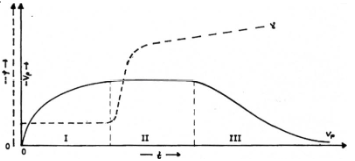
\includegraphics[scale = 0.75]{Bilder/Graph_Polymges.png}
				\caption{Dieser Graph zeigt die Polymerisationsgeschwindigkeit und die Oberflächenspannung im bezug auf die Zeit. \cite{polyskript}}
				\label{PolyGes}
			\end{figure}
			
		Der Abluauf der Polymerisation erfolgt, dass zu begin zum einen leere Mizellen vorliegen aber auch nur mit Monomer gefüllte Mizellen Vorliegen.
		Aus diesen, auch Monomertröpfchen genannte Mizellen diffundieren Monomere in die Leeren Mizellen. 
		Der anschließend zugefügte wasserlösliche Initiator zerfällt in der Lösung und die Radikale können in die Mizellen diffundieren. Dort findet der start der Polymerisation statt. 
		Wichtig hierbei ist das die anzahl der Monomertröpfchen duetlich kleiner ist als die anzahl der Mizellen wodurch eine statistische höhere diffusion in diese Stattfindet.
		Ist die Polymerisation gestartet wird Monomer verbraucht, dadurch steigt wie in Phase eins die Polymerisationsgeschwindigkeit an.
		Anschließend diffundieren weitere Monomere aus den Monomertröpfchen in die Mizelle wodurch die Polymerisationsgeschwindigkeit zunächst konstant bleibt (Phase 2).
		Ist diese "Monomerreserve" aufgebraucht nimmt auch die Monomermenge in der Mizelle langsam ab, wodurch auch die Polymerisationsgeschwindigkeit abnimmt (Phase 3).

	\subsection{Kinetik}

		Der Umsatz der Emulsionspolymerisation kann über folgende Gleichung berechnet werden:

			\begin{equation}
				U = \frac{m_\text{Feststoff}}{m_\text{M0}} \cdot \frac{1}{1 + \frac{m_\text{E0}}{m_\text{M0}}}\cdot \frac{m_\text{ges}}{m_\text{Probe}} \cdot 100\%
				\label{Umsatz}
			\end{equation}

		Dabei ist $m_\text{Feststoff}$ die Masse des Feststoffs, $m_\text{E0}$ die Masse des eingesetzten Emulgators, 
		$m_\text{MK0}$ die Masse des Monomers, $m_\text{ges}$ die Gesamtmasse des Ansatzes und $m_\text{Probe}$ ist die masse der Probe.
		


\section{Durchführung}

	Es wurden \SI{48}{mL} Wasser in einem Kolben vorgelegt. Hierzu wurde \SI{1,2}{g} Emulgator und \SI{12}{g} Styrol zugegeben. 
	Es wurde auf 70°C erhitzt und unter Rückfluss gerührt. Nach etwas \SI{30}{min} wurde eine vorbereitete Kaliumperoxodisulfat-Lösung (\SI{139}{mg} in \SI{4}{mL} Wasser) zugegeben.
	Im laufe der nächsten Drei stunden wurde zu in Tabelle \ref{Messwerte} zeitpunkten \SI{2}{mL} der Reaktionslösung entnommen und zu \SI{1}{mL} einer bereits hergestellten Hydrochinonlösung zugegeben.
	Diese werden in einem Hochvakuumschrank getrocknet und anschließend gewogen. wopbei das gewicht vor und nach trocknen notiert wird.

\section{Auswertung}

	\begin{table}[h]
    \centering
    \small % Schriftgröße leicht verringern
    \setlength{\tabcolsep}{4pt} % Horizontalen Abstand zwischen Spalten verringern
    \caption{Gemessene Massen, berechnete Umsätze und Reaktionsgeschwindigkeiten.}
    \label{Messwerte}
    \begin{tabular}{@{} r l c c c c c c r @{}}
        \toprule
        \textbf{t} & \textbf{Nr.} & \textbf{m1} & \textbf{m2} & \textbf{m2-m1} & \textbf{m3} & \textbf{m3-m1} & \textbf{Umsatz} & \textbf{$v_\text{Br}$} \\ 
        {[min]} & & {[g]} & {[g]*} & {[g]} & {[g]**} & {[g]} & {[\%]} & {[\%/min]} \\ \midrule
        2   & E1  & 10,8270 & 13,9534 & 3,1264 & 10,9110 & 0,0840 & 12,59 & 0,0002 \\
        4   & E2  & 10,7778 & 13,7803 & 3,0025 & 10,8348 & 0,0570 & 8,90  & 0,0002 \\
        6   & E3  & 10,8299 & 14,0035 & 3,1736 & 10,8998 & 0,0699 & 10,32 & 0,0002 \\
        10  & E4  & 10,8514 & 13,8913 & 3,0399 & 10,9106 & 0,0592 & 9,13  & 0,0003 \\
        15  & E5  & 10,7545 & 13,8498 & 3,0953 & 10,8220 & 0,0675 & 10,22 & 0,0004 \\
        20  & E6  & 10,8480 & 13,5827 & 2,7347 & 10,9018 & 0,0538 & 9,22  & 0,0005 \\
        30  & E7  & 10,8566 & 13,8379 & 2,9813 & 10,9099 & 0,0533 & 8,38  & 0,0008 \\
        45  & E8  & 10,8530 & 13,8975 & 3,0445 & 10,9102 & 0,0572 & 8,80  & 0,0019 \\
        60  & E9  & 10,7899 & 13,9295 & 3,1396 & 10,8568 & 0,0669 & 9,99  & 0,0042 \\
        90  & E10 & 10,7232 & 13,6237 & 2,9005 & 10,7862 & 0,0630 & 10,18 & 0,0212 \\
        120 & E11 & 10,8127 & 13,7319 & 2,9192 & 10,8863 & 0,0736 & 11,82 & 0,1067 \\
        150 & E12 & 10,8992 & 13,8830 & 2,9838 & 11,0244 & 0,1252 & 19,66 & 0,5377 \\
        180 & E13 & 10,9689 & 14,0060 & 3,0371 & 11,3577 & 0,3888 & 59,99 & 2,7100 \\ 
        \bottomrule
    \end{tabular}
\end{table}

	Wie in Tabelle \ref{Messwerte} bereits berechnet konnten die Umsätze bereits bestimmt werden.
	Diese können auf auf die Zeit geplottet werden woraus folgender Graph erhalten wird:

		\begin{figure}[H]
			\centering
			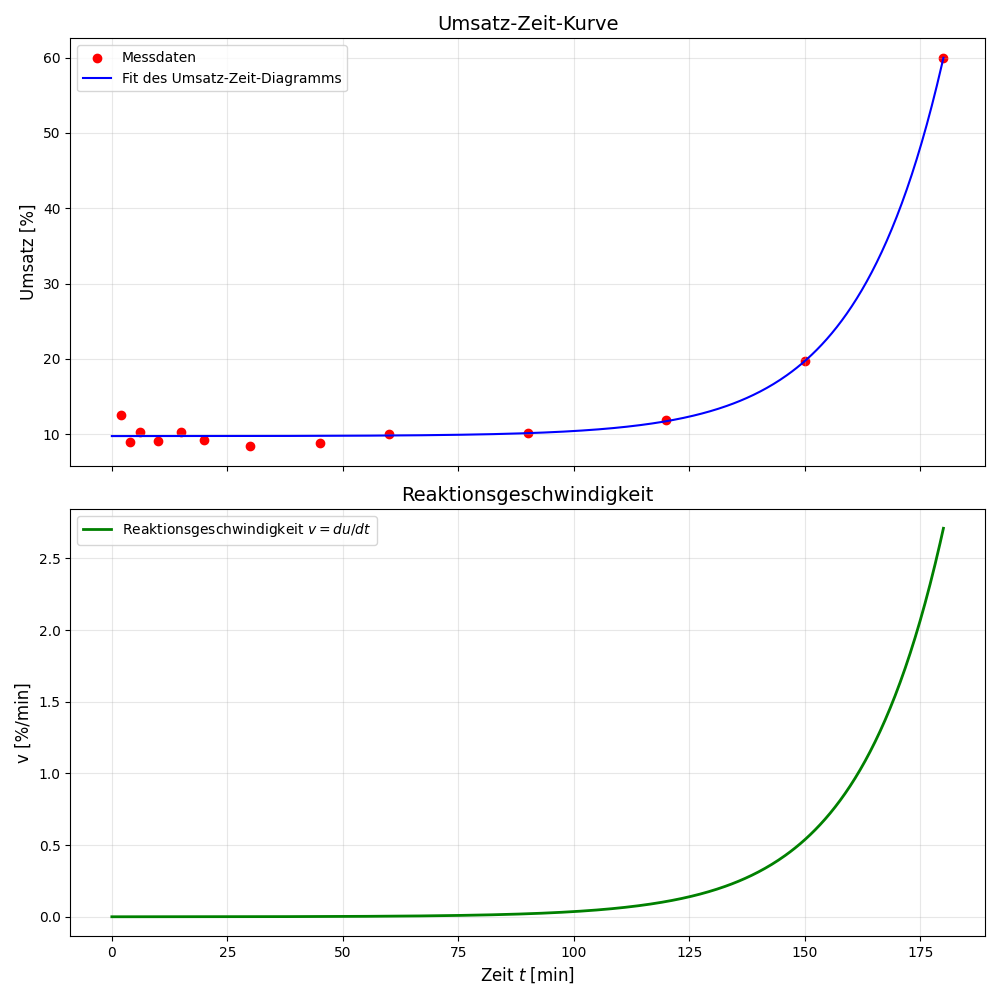
\includegraphics[scale = 0.5]{Bilder/UmsatzZeitPlot.png}
			\caption{Die Abbildung zeigt den Umsatz in \% aufgetragen auf die Reaktionsdauer.}
			\label{ZeitUmsatz}
		\end{figure}

	Aus  Abb. \ref{ZeitUmsatz} wird deutlich, dass der Umsatz nach einer bestimmten Zeit deutlich zunimmt, was nicht sein kann.
	Da wie oben bereits angesprochen der Umsatz zunächst stark zunehmen sollte und dann abflachen sollte. 
	Die vorleigenden Werte können falsch sein da vielleicht etwas bei der entnahme flasch gelaufen ist oder die reaktion nicht richtig gestartet ist.
	Folglich sind auch die Reaktionsgeschwindigkeiten nicht richtig wie aus Tabelle \ref{Messwerte} entnommen werden kann.
	Diese sollte auch zunächst stark steigen und dann abflachen.
	

\section{Fragen}

	\subsection{Frage 1}

		Durch die Anwesenheut von sauerstoff kann ein Kettenabbruch stattfinden da es sich trotz Emulsionspolymerisation rein Chemisch um eine radikalische Polymerisation handelt.
		Daraus folgt ein zusätzlicher anstieg der Polymerisationsgeschwindigkeit, da durch verbrauchen des Polymers die wahrscheinlichkeit steigt, dass eine Reaktion mit Sauerstoff stattfindet.

			
	\subsection{Frage 2}

		Zum einen die Elektrostatische Stabilisierung, dies ist vor allem bei anionischen Emulgatoren der fall. Alle der Teilchen erhalten die selbe ladung und können sich gegenseitig abstoßen.
		%Sterische Stabilisierung, Emulgatorkonz, Geringe Ionenstärke laut Gemini lol


	\subsection{Frage 3}

		Hierbei gilt das 1 oder 0 Prinzip. Nach diesem Prinzip ist im Latexteilchen entweder ein Radikal oder keines.
		Da im fall von zwei Radikalen, diese direkt rekombinieren würden und folglich kein Radikal übrig wäre.
		Daher folgt 0,5 als durchschnittliche anzah an Radikalen.

	\subsection{Frage 4}
		
		Das grundlegende Konzept eines Redoxinitiators ist das erzeugen eines Radikals durch ein-Elektron Übertragung.
		So wird im beispiel von Eisen(II)-Peroxodisulfat Eisen Oxidiert und im laufe der Oxidation entsteht ein Sulfat und ein Sulfat-Radikalanion.

			\begin{equation}
				\ch{S2O8^2- + Fe^{2+} -> SO4^2- + SO4^{-}. + Fe^{3+}}
			\end{equation}

		Der Vorteil dieser Initiatoren ist eine hohe kontrolle der Reaktionsgeschwindigkeit ohne hohe temperaturen anzuwenden.
		Es wird lediglich die Konzentration des Redox-Partners geändert.
		Ein Problem was deutlich wird, ist das Problem das sich die Radikale gut in wasser lösen und somit nicht direkt in die Mizelle kommen.
		Dabei wird mit dem Oligomer-Radikal-Modell gearbeitet. Dabei Startet ein Teil der Polymerisation beriets in der wässrigen Phase wobei sich Oligomere bilden welche den 
		hydrophielen charakter des Radikals ändern. 
		Dieses Oligomer gelangt anschließend in das Latexteilchen, wo es weiter polymerisiert.

	\subsection{Frage 5}

		Ein großer Unterschied zwischen diesen beiden Varianten ist die lösligkeit des Initiator.
		So ist bei der Emulsionspolymerisation der Initiator Wasserlöslich und bei der Suspensionspolymerisation Monomerlöslich.
		Anders ist auch der Ort der Reaktion so findet die Reaktion bei der Emulsionspolymerisation in der Latexzelle statt.
		Bei der Suspensionspolymerisation findet diese in den Monomertröpfchen statt.
		Ein weiterer großer unterschied ist die teilchengröße, so sind die teichen der Emulsionspolymerisation kleiner als die der Suspensionspolymerisation.
		Weitere Polymerisationsmethoden sind zum Beispiel die Lösungspolymerisation, die Fällungspolymerisation und die Gasphasenpolymerisation.

\printbibliography

\end{document}